\section{Modelli probabilistici di diffusione del rumore (DDPM) }


I modelli probabilistici di diffusione del rumore (DDPM) sono stati introdotti in un articolo pubblicato nell'estate del 2020 (Ho et al.,~\cite{ho2020}) 
che ha segnato un punto di svolta nell'ambito dei modelli di diffusione e della modellazione generativa.

\medskip
\noindent La \emph{pipeline} di un DDPM è la seguente:
\begin{itemize}
\item nel \emph{processo di diffusione in avanti}, un'immagine è corrotta dal rumore fino a risultare, all'acme del processo, indistinguibile dallo stesso. 
La diffusione in avanti è funzionale a ricondursi, da un distribuzione di probabilità arbitrariamente complessa dell'immagine di partenza, al rumore puro che, invece, esibisce una distribuzione nota e 
facilmente manipolabile.
\item nel \emph{processo di diffusione inversa}, con l'ausilio di una rete neurale, si rimuove progressivamente il rumore, ripercorrendo a ritroso la diffusione in avanti, fino a pervenire all'immagine scevra da rumore. 
\end{itemize}


\subsection{Processo di diffusione in avanti}

Il processo di diffusione in avanti (\emph{forward diffusion process}) è definito come una \emph{catena markoviana} (si veda~\ref{ssec:markov_chain})
che va a perturbare la distribuzione originale, incognita, $q(\mathbf{x}_0)$ di un'immagine $\mathbf{x}_0$ del dataset di addestramento, 
corrompendola con rumore additivo gaussiano (Figura~\ref{fig:forward_diff_process}).

Qualora il suddetto rumore additivo abbia entità contenuta, le \emph{transizioni} della catena markoviana nel processo di diffusione in avanti possono essere 
modellate come distribuzioni gaussiane condizionate (Ho et al., $2020$~\cite{ho2020}). Avvalendosi del formalismo matematico risulta che:
\smallskip
\begin{Mybox1}
\begin{align}
  q(\mathbf{x}_{1:T}|\mathbf{x}_0)  & \triangleq \prod\limits_{t=1}^{T}q(\mathbf{x}_t|\mathbf{x}_{t-1})\quad\quad \text{Processo di diffusione in avanti} \label{eq:forward_process}\\
  q(\mathbf{x}_t | \mathbf{x}_{t-1}) & \triangleq \mathcal{N}(\mathbf{x}_t; \sqrt{1-\beta_t}\mathbf{x}_{t-1},\beta_t \bm{I}) \quad\quad  \text{Generica transizione}\label{eq:forward_chain_transition}
\end{align}
\end{Mybox1}
\smallskip
\noindent dove
\begin{itemize}
  \item $t\in[1,\dots,T]$ è il generico passo temporale.
  \item $\{\beta_t \in (0,1)\}_{t=1}^T$ implementano uno \hyperref[sssec:diff_schedules]{\emph{schema di diffusione}}.
  \item $\mathbf{x}_t$ è l'immagine a valle della $t$-esima transizione della diffusione in avanti.
  \item $\mathbf{x}_0$ è l'immagine originale di partenza che, dopo $T$ passi,
  converge a $\mathbf{x}_T$.
\end{itemize}
\bigskip
\noindent La~\eqref{eq:forward_chain_transition}, in virtù dell'\emph{artificio di riparametrizzazione} 
(si veda~\eqref{eq:rep_trick}), è equivalente ad asserire che
\begin{equation}\label{eq:rep_chain_transition}
 \mathbf{x}_t = \sqrt{1-\beta_t}\mathbf{x}_{t-1} + \sqrt{\beta_t}\bm{\epsilon}_{t-1} 
\end{equation}
dove $\bm{\epsilon}_{t-1} \sim \mathcal{N}(\mathbf{0},\bm{I})$.
\begin{oss}
  Si osserva esplicitamente che, nella~\eqref{eq:forward_chain_transition}, $\mathbf{x}_{t-1}$ è \emph{fissato}:
  il vettore  $\sqrt{1-\beta_t}\mathbf{x}_{t-1}$ è, quindi, \emph{deterministico}.
  Pertanto, dalla~\eqref{eq:forward_chain_transition} si evince che l'immagine $\mathbf{x}_t$ è distribuita come 
  una gaussiana condizionata con media $\bm{\mu}_t=\sqrt{1-\beta_t}\mathbf{x}_{t-1}$ e varianza $\bm{\Sigma}_t=\beta_t\bm{I}$.
\end{oss}
\medskip
\noindent Dalla~\eqref{eq:rep_chain_transition} si desume \emph{come} si ottiene l'immagine al passo 
temporale corrente $\mathbf{x}_t$ a partire dall'immagine $\mathbf{x}_{t-1}$ allo stato
precedente: ad una versione scalata di quest'ultima si aggiunge rumore gaussiano scalato.
Avendo l'accortezza di scegliere i $\beta_t$ opportunamente, si perverrà ad un'immagine $\mathbf{x}_T$ che, per $T$ sufficientemente elevato, 
approssima una distribuzione gaussiana standard ed è, pertanto, indistinguibile dal rumore gaussiano puro~\cite{ho2020}.
\begin{figure}
  \centering
  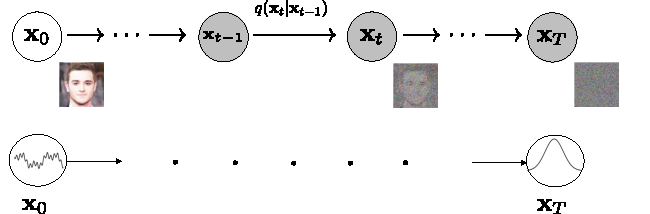
\includegraphics[keepaspectratio]{forward_process2456.pdf} 
  \caption{Processo di diffusione in avanti. Fonte~\cite{ho2020}.} \label{fig:forward_diff_process}
\end{figure}
\medskip
\begin{oss}
Il passaggio dalla~\eqref{eq:forward_chain_transition} alla~\eqref{eq:rep_chain_transition}, ricorrendo all'artificio di 
riparametrizzazione, sarà un \emph{pattern} ricorrente nel prosieguo, in particolare nella riformulazione del processo di diffusione in avanti 
atta a pervenire ad una versione ottimizzata dello stesso.
\end{oss}
\begin{oss}
  Il numero totale degli step di diffusione $T$ è un \emph{iperparametro} e, in quanto tale, 
  va fissato a monte della fase di addestramento del modello. Ho et al.\ ($2020$~\cite{ho2020}) hanno 
  propeso per $T=1000$. 
\end{oss}
\begin{oss}
  È importante osservare che, poiché ad ogni transizione della catena markoviana in avanti viene aggiunto solo del rumore, il
  processo di diffusione in avanti risulta \emph{fissato} qualora si scelgano i $\beta_t$.
\end{oss}
\medskip
\noindent Ricapitolando, il processo di diffusione in avanti trasforma, mediante l'aggiunta progressiva di rumore gaussiano, 
la complessa distribuzione incognita $q(\mathbf{x}_0)$ iniziale in una distribuzione normale standardizzata $\mathcal{N}(\bm{0},\bm{I})$. Il punto 
di forza di una siffatta distribuzione è insito nel suo essere facilmente manipolabile.
La distribuzione terminale della diffusione in avanti costituisce il punto di partenza del processo di diffusione inversa.



\subsubsection{Implementazione del processo di diffusione in avanti}

A beneficio di una maggiore ricchezza argomentativa, nonché per avere un riscontro pratico di 
quanto esposto precedentemente, viene riportata una possibile implementazione del processo di 
diffusione in avanti, partendo da una mia fotografia.

\begin{lstlisting}[language=iPython, caption=Codice adattato da~\cite{nain2022} e implementato con Google Colab~\cite{GoogleColaboratory},label=lst:diff]
import numpy as np                   # per manipolare array e matrici 
from PIL import Image                # per manipolare le immagini  
from matplotlib import pyplot as plt # per creare e visualizzare grafici 
from google.colab import files       # per scaricare l'immagine finale
  
def forward_diff_process(img_t_meno_(*@\color{black}{1}@*), beta, t):
    """
    Tale funzione implementa la generica transizione dall'immagine
    al passo t-1 all'immagine al passo t del processo di diffusione
    in avanti.

    Input:
        img_t_meno_1: immagine al passo precedente (*@$\mathcolor{ipython_red}{(\mathbf{x}_{t-1})}$@*)
        beta: schema di diffusione (vettore di numeri)
        t: passo corrente 
    Output:
        img_t: immagine a valle della transizione (*@$\mathcolor{ipython_red}{(\mathbf{x}_t)}$@*)
    """

    # 1. Si ricava (*@$\mathcolor{ipython_green}{\beta_t}$@*)
    beta_t = beta[t].reshape(-1, 1, 1)  

    # 2. Calcolo media statistica e deviazione standard
    mu = np.sqrt((1.0 - beta_t)) * img_t_meno_(*@\color{black}{1}@*)
    sigma = np.sqrt(beta_t)

    # 3. Generazione dell'immagine al passo t tramite l'equazione(*@\color{ipython_green}{~\eqref{eq:rep_chain_transition}}@*)
    img_t = mu + sigma*np.random.randn(*img_t_meno_(*@\color{black}{1}@*).shape)
    return img_t  

# ------------------------------------------------------------
# Esempio di applicazione del processo di diffusione in avanti  
# ------------------------------------------------------------

# 1. Si carica l'immagine di partenza (*@\color{ipython_green}{$\mathbf{x}_0$}@*)
img = Image.open("../content/selfie.jpg")

# 2. Si ridimensiona l'immagine secondo le dimensioni desiderate
IMG_SIZE = (100, 172)
img = img.resize(size=IMG_SIZE)

# 3. Si definisce il numero dei passi temporali (T)
timesteps = 100

# 4. Implementazione schema di diffusione lineare
beta_start = 0.0001
beta_end = 0.05
beta = np.linspace(beta_start, beta_end, num=timesteps, dtype=np.float(*@\color{black}{32}@*))

immagini_processate = [] 
img_t = np.asarray(img.copy(), dtype=np.float(*@\color{black}{32}@*)) / 255.

# 5.  Esecuzione del processo di diffusione in avanti
#     per ottenere l'immagine a valle di (*@$\mathcolor{ipython_green}{T=100}$@*) passi
for t in range(timesteps):   (*@\label{line:fw_diff}@*)                                                                
    img_t = forward_diff_process(img_t_meno_(*@\color{black}{1}@*)=img_t, beta=beta, t=t)
    if t%20==0 or t==timesteps - 1:   
        immagine = (img_t.clip(0, 1) * 255.0).astype(np.uint(*@\color{black}{8}@*))
        immagini_processate.append(immagine) (*@\label{line:fw_diff1}@*)

# 6. Visualizzazione delle immagini per diversi passi di diffusione
_, ax = plt.subplots(1, len(immagini_processate), figsize=(15, 8))

for i, immagine in enumerate(immagini_processate):
    ax[i].imshow(immagine)
    ax[i].set_title((*@\color{blue}{f}@*)"Timestep: (*@\color{ipython_green}{\{}\color{black}{i}\color{ipython_purple}{*}\color{black}{20}\color{ipython_green}{\}}@*)",fontsize=18)
    ax[i].axis("off")
    ax[i].grid(False)

plt.suptitle("Processo di diffusione in avanti", fontsize=22, y=0.78)
plt.savefig("forward_diff.pdf",pad_inches=0,bbox_inches='tight')
files.download('forward_diff.pdf')
plt.show()
plt.close()
\end{lstlisting}
\smallskip
\begin{center}
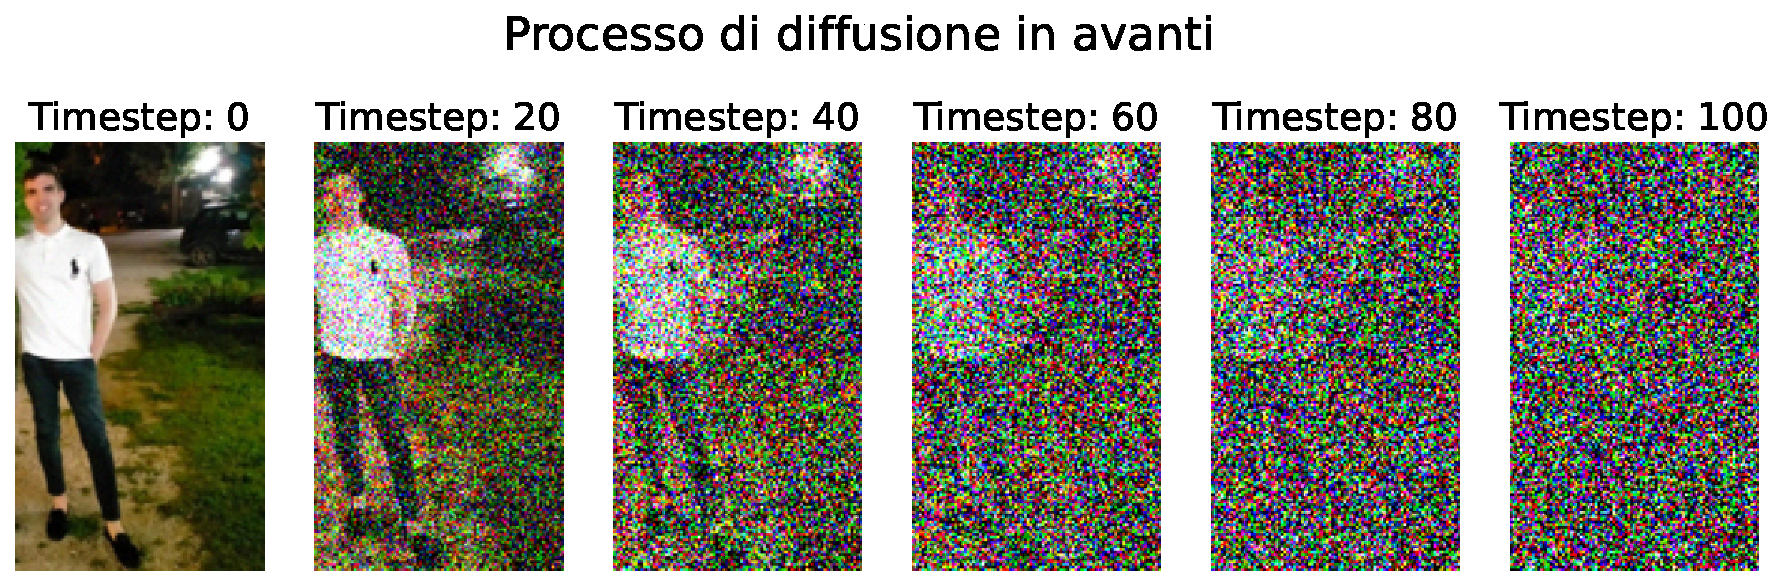
\includegraphics[keepaspectratio, scale=0.4]{code_result.pdf}
\end{center}

\noindent Si noti la progressiva perdita di connotati dell'immagine di partenza che, a valle di 
$T$ passi di diffusione, risulta indistinguibile dal rumore puro. 


%--------------------------------------------------------------

\subsubsection{Ottimizzazione del processo di diffusione in avanti}


Da un'attenta analisi del codice~\ref{lst:diff}, in particolare dalla riga~\ref{line:fw_diff} alla riga~\ref{line:fw_diff1}, si evince 
che, per pervenire all'immagine terminale $\mathbf{x}_T$, è necessario simulare l'\emph{intera} catena markoviana della diffusione in avanti:
all'aumentare del numero di step totali $T$ ciò risulta fortemente inefficiente.
Per ovviare a tale problema, definendo preliminarmente
\begin{equation}
  \alpha_t \triangleq  1-\beta_t, \quad\quad \overline{\alpha}_t  \triangleq \prod\limits_{i=1}^{t}\alpha_i \label{eq:alphas}
\end{equation} 
Ho et al.~\cite{ho2020} hanno osservato che la~\eqref{eq:rep_chain_transition} ammette la seguente riformulazione:
\begin{align}
\mathbf{x}_t & = \sqrt{1-\beta_t}\mathbf{x}_{t-1}+\sqrt{\beta_t}\bm{\epsilon}_{t-1}  \label{eq:eff_forward1}   \\ 
             & = \sqrt{\alpha_t}\mathcolor{blue}{\mathbf{x}_{t-1}}+\sqrt{1-\alpha_t}\bm{\epsilon}_{t-1}  \label{eq:eff_forward2}   \\ 
             & = \sqrt{\alpha_t}\bigl(\mathcolor{blue}{\sqrt{\alpha_{t-1}}\mathbf{x}_{t-2}+\sqrt{1-\alpha_{t-1}}\bm{\epsilon}_{t-2}}\bigr) + \sqrt{1-\alpha_t}\bm{\epsilon}_{t-1} \label{eq:eff_forward3}\\
             & = \sqrt{\alpha_t\alpha_{t-1}}\mathbf{x}_{t-2}+\mathcolor{red}{\sqrt{\alpha_t(1-\alpha_{t-1})}\bm{\epsilon}_{t-2}+\sqrt{1-\alpha_t}\bm{\epsilon}_{t-1}} \label{eq:eff_forward4}\\ 
             & = \sqrt{\alpha_t\alpha_{t-1}}\mathbf{x}_{t-2} + \mathcolor{red}{\sqrt{1-\alpha_t\alpha_{t-1}}\overline{\bm{\epsilon}}_{t-2}} \label{eq:eff_forward5} \\
             & = \dots \\
             & = \sqrt{\alpha_t\alpha_{t-1}\dots\alpha_1}\mathbf{x}_0 + \sqrt{1-\alpha_t\alpha_{t-1}\dots\alpha_1}\bm{\epsilon}_0 \\
             & = \sqrt{\overline{\alpha}_t}\mathbf{x}_0+\sqrt{1-\overline{\alpha}_t}\bm{\epsilon}_0, \label{eq:eff_forward}  
\end{align}

\noindent dove:
\begin{itemize}
  \item $\{\overline{\bm{\epsilon}}_{t},\bm{\epsilon}_{t}\}_{t=0}^T\overset{\text{iid}}{\sim} \mathcal{N}(\bm{0},\bm{I})$.
  \item dalla~\eqref{eq:eff_forward2} alla~\eqref{eq:eff_forward3} ci si è avvalsi dell'artificio di 
        riparametrizzazione~\eqref{eq:rep_trick}.
  \item il passaggio dalla~\eqref{eq:eff_forward4} alla~\eqref{eq:eff_forward5} è il combinato disposto dell'artificio di riparametrizzazione e 
  del risultato per cui una combinazione lineare di vettori gaussiani 
  \emph{indipendenti} è ancora un vettore gaussiano~\eqref{eq:comblingauss_scalar}. Infatti, poiché
  \begin{align}
    \sqrt{1-\alpha_t}\bm{\epsilon_{t-1}} &\sim \mathcal{N}(\bm{0},(1-\alpha_t)\bm{I}) \label{eq:rep_trick1}\\
    \sqrt{\alpha_t(1-\alpha_{t-1})}\bm{\epsilon_{t-2}} &\sim \mathcal{N}(\bm{0},(\alpha_t-\alpha_t\alpha_{t-1})\bm{I}) \label{eq:rep_trick2}
  \end{align}
  ed essendo $\bm{\epsilon_{t-1}}$ ed $\bm{\epsilon_{t-2}}$ \emph{indipendenti}, la somma di~\eqref{eq:rep_trick1} e~\eqref{eq:rep_trick2} è distribuita come
  \[
    \mathcal{N}(\bm{0},(1-\alpha_t+\alpha_t-\alpha_t\alpha_{t-1})\bm{I})=\mathcal{N}(\bm{0},(1-\alpha_t\alpha_{t-1})\bm{I})
  \]
  il che, ricorrendo all'artificio di riparametrizzazione, equivale a:
  \[
    \sqrt{1-\alpha_t}\bm{\epsilon_{t-1}} + \sqrt{\alpha_t(1-\alpha_{t-1})}\bm{\epsilon_{t-2}}
    =\sqrt{1-\alpha_t\alpha_{t-1}}\overline{\bm{\epsilon}}_{t-2}
  \]
\end{itemize} 

\begin{figure}
  \centering
  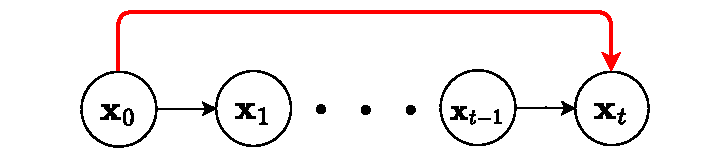
\includegraphics[keepaspectratio, scale=0.8]{forward_process3.pdf}
  \caption{Passaggio diretto da $\mathbf{x}_0$ a $\mathbf{x}_t$. Fonte:~\cite{vaibhavsinghInDepthGuideDenoising2023}.}
 \label{fig:skip_steps}
\end{figure}

\noindent Pertanto, il processo di diffusione in avanti può essere così riformulato:
\begin{Mybox}
\begin{equation}
  q(\mathbf{x}_t|\mathbf{x}_0)=\mathcal{N}\bigl(\mathbf{x}_t;\sqrt{\overline{\alpha}_t}\mathbf{x}_0,(1-\overline{\alpha}_t)\bm{I}\bigr) \label{eq:forward_diff_v2}
\end{equation}
\end{Mybox}
\smallskip
\noindent La riformulazione~\eqref{eq:forward_diff_v2} del processo di diffusione in avanti, basata 
essenzialmente sull'applicazione ricorsiva dell'artificio di riparametrizzazione, apporta un duplice beneficio:
\begin{itemize}
\item dall'immagine di partenza $\mathbf{x}_0$ è possibile raggiungere un $\mathbf{x}_t$ \emph{qualsiasi} con un \emph{unico} step di diffusione in avanti (Figura~\ref{fig:skip_steps}).
\item per progettare uno \emph{schema di diffusione} è possibile avvalersi degli $\overline{\alpha}_t$, in luogo dei $\beta_t$ originali. Il vantaggio di ciò 
risiede nell'interpretazione di $\overline{\alpha}_t$ come la varianza del segnale (l'immagine di partenza $\mathbf{x}_0$) e 
$1-\overline{\alpha}_t$ come la varianza del rumore $\bm{\epsilon}$~\cite{fosterGenerativeDeepLearning2023}.
\end{itemize} 

\noindent Si riporta di seguito l'implementazione della versione ottimizzata del processo di diffusione in avanti, 
per corroborare la perfetta equivalenza sussistente tra le due formulazioni dello stesso, precedentemente investigate.


\begin{lstlisting}[language=iPython,caption=Diffusione in avanti ottimizzata. Codice adattato da~\cite{nain2022},label=lst:diff_ott]
import numpy as np                 
from PIL import Image             
from matplotlib   import pyplot as plt   
from google.colab import files     
    
def forward_diff_process_ott(img_orig, alpha_bar, t):
    """
    Input:
        img_orig: immagine al passo t=0 (*@$(\mathcolor{ipython_red}{\mathbf{x}_0})$@*)
        alpha_bar: versione riparametrizzata di beta
        t: passo corrente 
    Output:
        img_t: immagine ottenuta al passo corrente (*@$(\mathcolor{ipython_red}{\mathbf{x}_t})$@*)
    """
    
    # 1. Si ricava (*@$\mathcolor{ipython_green}{\overline{\alpha}_t}$@*)
    alpha_bar_t = alpha_bar[t].reshape(-1, 1, 1)
    
    # 2. Calcolo media statistica e deviazione standard
    mu = np.sqrt(alpha_bar_t) * img_orig
    sigma = np.sqrt(1.0 - alpha_bar_t)
    
    # 3. Generazione dell'immagine al passo t tramite l'equazione(*@\color{ipython_green}{~\eqref{eq:eff_forward}}@*)
    img_t = mu + sigma * np.random.randn(*img_orig.shape)
    return img_t
  

# 1. Si carica l'immagine di partenza (x0) 
img = Image.open("../content/selfie.jpg")
  
# 2. Si ridimensiona l'immagine secondo le dimensioni desiderate
IMG_SIZE = (100, 172)
img = img.resize(size=IMG_SIZE)
  
# 3. Si definisce il numero dei passi temporali (T)
timesteps = 100

#----------------------------------------------------------
# Versione ottimizzata del processo di diffusione in avanti  
#----------------------------------------------------------

# 4. Implementazione schema di diffusione lineare
beta_start = 0.0001
beta_end = 0.05
beta = np.linspace(beta_start, beta_end, num=timesteps, dtype=np.float32)

# 5. Si definiscono alpha e alpha_bar secondo la (*@\color{ipython_green}{\eqref{eq:alphas}}@*)
alpha = 1.0 - beta
alpha_bar = np.cumprod(alpha)
  
immagini_processate = [img] # immagine (*@$\mathcolor{ipython_green}{\mathbf{x}_0}$@*)
img_orig = np.asarray(img.copy(), dtype=np.float32) / 255.

# 6. Esecuzione del passo di diffusione in avanti per timestep specifici
# Si scelgono gli stessi timestep visualizzati nel codice (*@\color{ipython_green}{\ref{lst:diff}}@*)
timestep_specifici = [19, 39, 59, 79, 99]
for step in timestep_specifici:
    img_t = forward_diff_process_ott(img_orig, alpha_bar, step)
    img_t = (img_t.clip(0, 1) * 255.0).astype(np.uint8)
    immagini_processate.append(img_t)
  

# 7. Visualizzazione delle immagini in diversi passi di diffusione
_, ax = plt.subplots(1, len(immagini_processate), figsize=(15, 8))

for i, sample in enumerate(immagini_processate):
    ax[i].imshow(sample)
    ax[i].set_title((*@\color{blue}{f}@*)"Timestep: (*@\color{ipython_green}{\{}\color{black}{i}\color{ipython_purple}{*}\color{black}{20}\color{ipython_green}{\}}@*)",fontsize=18)
    ax[i].axis("off")
    ax[i].grid(False)

plt.suptitle("Diffusione in avanti ottimizzata",fontsize=22, y=0.78)
plt.savefig("forward_process_v2.pdf",pad_inches=0,bbox_inches='tight')
files.download('forward_process_v2.pdf')
plt.show()
plt.close()
\end{lstlisting}
\begin{center}
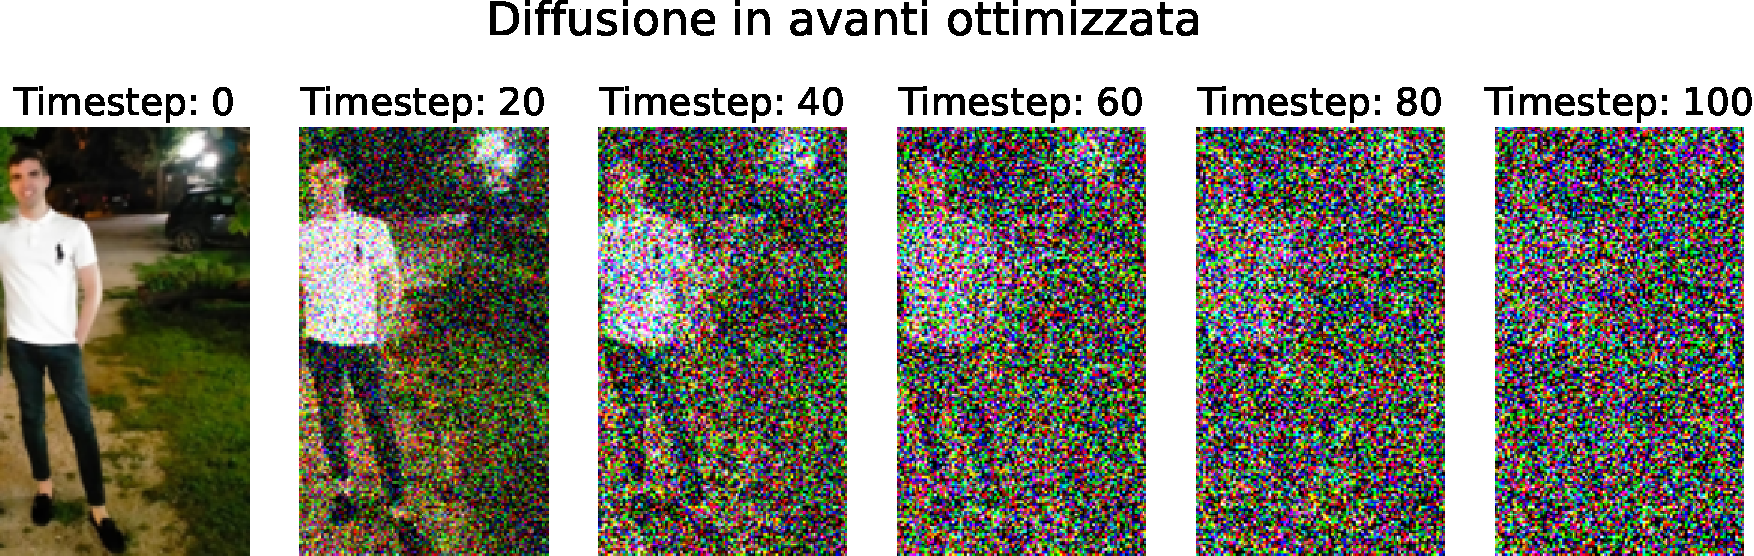
\includegraphics[keepaspectratio, scale=0.4]{efficient_forward_process.pdf}
\end{center}
Si noti che, sebbene il risultato del codice~\ref{lst:diff_ott} sia il medesimo del codice~\ref{lst:diff}, il discrimine tra i due è 
insito nel \emph{modo} in cui si perviene alle immagini nei diversi passi di diffusione.

%---------------------------------------------------------------------
\subsubsection{Schemi di diffusione}\label{sssec:diff_schedules}

\begin{figure}
  \centering
  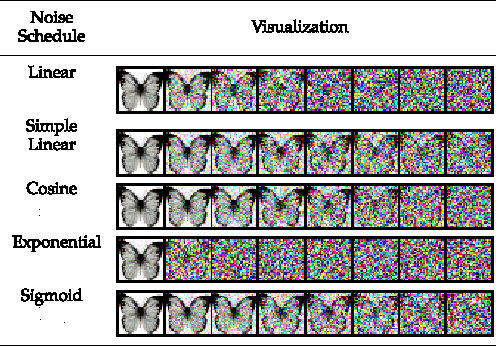
\includegraphics[keepaspectratio, scale=0.9]{diff_schedules}
  \caption{Diversi schemi di diffusione. Fonte:~\cite{changDesignFundDiffusion2023}.}
  \label{fig:diff_schedules}
\end{figure}

Uno schema di diffusione si esplica in una particolare istanza del 
vettore\footnote{Abuso di notazione: l'apice $T$ è l'operazione di \emph{trasposizione},
il pedice $T$ è il numero totale degli step di diffusione.} $\bm{\beta}=(\beta_1,\dots,\beta_T)^T$, e controlla la quantità di rumore 
che viene aggiunta ad ogni passo della catena markoviana nel processo di diffusione in avanti.

\bigskip
\noindent In letteratura si ravvisano due approcci:
\begin{itemize}
\item si addestra una rete neurale ad apprendere i $\beta_t$ che, in tal caso, sono considerati alla stregua di 
parametri ordinari della rete.
Perseguendo tale approccio è possibile implementare schemi di diffusione \emph{diversi} per la fase di addestramento 
e la fase di inferenza~\cite{changDesignFundDiffusion2023}.
\item i $\beta_t$ assurgono ad iperparametri e, in quanto tali, sono fissati a priori (\emph{hyperparameter tuning}). In 
tal caso, per progettare i $\beta_t$, in letteratura, si ricorre ad un ampio ventaglio di tecniche \emph{euristiche}~\cite{changDesignFundDiffusion2023}.
\end{itemize}
Ho et al.~\cite{ho2020} hanno optato per quest'ultimo approccio, propendendo per uno schema di diffusione \emph{lineare} 
in cui i $\beta_t$ crescono linearmente da $\beta_1=10^{-4}$ a $\beta_T=0.02$.

Tuttavia, è stato dimostrato (Nichol et al., $2021$~\cite{nicholImprovedDenoisingDiffusion2021a}) 
che l'impiego di uno schema di diffusione sinusoidale implica un incremento delle prestazioni del modello di diffusione.
In Figura~\ref{fig:diff_schedules} sono riportati diversi schemi di diffusione.

Nel progettare uno schema di diffusione non si deve trascurare l'ingrediente fondamentale nel deep learning: i \emph{dati}.
Dal punto di vista della rappresentazione dei dati, la dimensionalità degli stessi e la massima distanza euclidea tra i campioni di addestramento 
sono fattori da contemplare nel design di uno schema di diffusione~\cite{songImprovedTechniquesTraining2020}. Inoltre, uno schema di diffusione deve 
tener conto della complessità e della ridondanza insita nei dati~\cite{chenImportanceNoiseScheduling2023}. Ad esempio, immagini più grandi potrebbero richiedere più 
rumore additivo, a parità di passi di diffusione in avanti, rispetto ad immagini di dimensioni più piccole~\cite{nicholImprovedDenoisingDiffusion2021a}.

Il \emph{tipo di rumore} aggiunto ad ogni passo del processo di diffusione in avanti è un altro iperparametro: Ho et al.~\cite{ho2020} hanno propeso 
per rumore gaussiano $\bm{\epsilon}\sim\mathcal{N}(\bm{0},\bm{I})$. 


\subsection{Processo di diffusione inversa}


La magia dei modelli di diffusione avviene nel processo di diffusione inversa (\emph{reverse diffusion process}). 
La \emph{ratio} sottesa al processo di diffusione inversa è quella di rimuovere iterativamente rumore
(\emph{denoising}) dall'immagine $\mathbf{x}_T\sim\mathcal{N}(\bm{0},\bm{I})$ (a cui si perviene a valle del processo di diffusione in avanti),
per risalire alla distribuzione incognita dell'immagine di partenza $q(\mathbf{x}_0)$ (Figura~\ref{fig:reverse_diff_process}).
Tuttavia per assolvere a tale scopo, il processo di diffusione inversa non può servirsi della distribuzione a posteriori
$q(\mathbf{x}_{t-1}|\mathbf{x}_t)$. Infatti, ricorrendo alla legge di Bayes~\eqref{eq:Bayes}, risulta che
\begin{equation}
    q(\mathbf{x}_{t-1}|\mathbf{x}_t)=\frac{q(\mathbf{x}_{t}|\mathbf{x}_{t-1})q(\mathbf{x}_{t-1})}{q(\mathbf{x}_t)} \label{eq:reverse_transition}
\end{equation}
da cui si evince come l'intrattabilità di $q(\mathbf{x}_{t-1}|\mathbf{x}_t)$ sia imputabile alle distribuzioni marginali $q(\mathbf{x}_{t-1})$ e $q(\mathbf{x}_t)$ 
in quanto~\footnote{Risultato analogo sussite \emph{mutatis mutandis} per $q(\mathbf{x}_{t-1})$}:
\begin{align}
    q(\mathbf{x}_t) &= \int q(\mathbf{x}_0,\mathbf{x}_1,\dots,\mathbf{x}_t)\,d\mathbf{x}_0\,d\mathbf{x}_1\dots\,d\mathbf{x}_{t-1} \label{eq:marginalization_op} \\
                    &= \int q(\mathbf{x}_1,\dots,\mathbf{x}_t|\mathbf{x}_0)q(\mathbf{x}_0) \,d\mathbf{x}_0\,d\mathbf{x}_1\dots\,d\mathbf{x}_{t-1} \label{eq:marginal}
\end{align}
dove $q(\mathbf{x}_1,\dots,\mathbf{x}_t|\mathbf{x}_0)$ è la catena markoviana della diffusione in avanti definita dalla~\eqref{eq:forward_process}, 
e nella~\eqref{eq:marginalization_op} si è effettuata l'operazione di marginalizzazione~\eqref{eq:marginalizzazione}.

Dalla~\eqref{eq:marginal} si evince chiaramente che il problema sotteso al calcolo di $q(\mathbf{x}_t)$ è duplice:
\begin{itemize}
\item la distribuzione $q(\mathbf{x}_0)$ è \emph{incognita}.
\item l'integrale nella~\eqref{eq:marginal}, essendo esteso ad uno spazio (di pixel) ad alta dimensionalità, è \emph{intrattabile}.
\end{itemize}
\begin{figure}
    \centering
    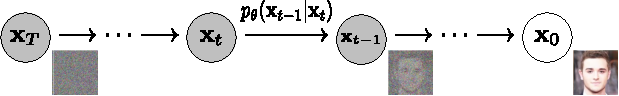
\includegraphics[keepaspectratio]{reverse_diff_process}
    \caption{Processo di diffusione inversa. Fonte:~\cite{ho2020}.}
    \label{fig:reverse_diff_process}
\end{figure}
Ho et al.~\cite{ho2020}, sulla scia di Sohl-Dickstein et al.~\cite{sohl-dickstein2015}, propongono l'addestramento di una rete neurale
per approssimare $q(\mathbf{x}_{t-1}|\mathbf{x}_t)$.

\noindent Il processo di diffusione inversa, quindi, è definito come un catena markoviana di transizioni gaussiane i cui parametri
(i.e.\ media e varianza) sono appresi 
da una rete neurale. L'assunzione di gaussianità per le suddette transizioni è supportata 
dall'osservazione che, qualora i $\beta_t$ abbiano entità contenuta, le transizioni di entrambi i processi 
di diffusione (diretta e inversa) esibiscono la stessa forma funzionale~\cite{fellerTheoryStochasticProcesses1949}.
Matematicamente risulta che:
\noindent 
\begin{Mybox1}
\begin{gather}
    p_{\bm{\theta}}(\mathbf{x}_{0:T})   \triangleq p(\mathbf{x}_T)\prod\limits_{t=1}^{T}p_{\bm{\theta}}(\mathbf{x}_{t-1}|\mathbf{x}_t) \, \text{Processo di diffusione inversa} \label{eq:reverse_process} \\
    p_{\bm{\theta}}(\mathbf{x}_{t-1}|\mathbf{x}_t) \triangleq \mathcal{N}(\mathbf{x}_{t-1}; \bm{\mu}_{\bm{\theta}}(\mathbf{x}_t,t),\bm{\Sigma}_{\bm{\theta}}(\mathbf{x}_t,t)) \,  \text{Generica transizione}\label{eq:chain_transition132}
\end{gather}
\end{Mybox1}
\noindent dove:
\begin{itemize}
\item $p(\mathbf{x}_T)=q(\mathbf{x}_T)=\mathcal{N}(\mathbf{x}_T;\bm{0},\bm{I})$ dal momento 
che il punto di arrivo della diffusione in avanti costituisce la base di partenza del processo di diffusione inversa.
\item il pedice $\bm{\theta}$ denota il vettore dei \emph{parametri} della rete neurale, aggiornati con la tecnica del gradiente discendente stocastico.
\item $\bm{\mu}_{\bm{\theta}}(\mathbf{x}_t,t)$,$\bm{\Sigma}_{\bm{\theta}}(\mathbf{x}_t,t)$ 
sono rispettivamente media e varianza che, come suggerisce la notazione (i.e il pedice $\bm{\theta}$), sono appresi dalla rete neurale.
\end{itemize}

\bigskip
\noindent Ricapitolando, il processo di diffusione inversa consiste nel rimuovere 
iterativamente (anziché in un singolo passo come le GAN~\cite{changDesignFundDiffusion2023}), servendosi di una rete neurale, 
il rumore dall'immagine $\mathbf{x}_T$. Tale processo di diffusione inversa è imbastito sull'immagine terminale della diffusione in avanti
e, al decrescere di $t$ da $T$ a $0$, si propaga nella direzione opposta a quest'ultima tramite una catena markoviana 
di transizioni~\eqref{eq:chain_transition132}.

\subsection{Addestramento}


Da quanto detto nel paragrafo precedente, \emph{si ricorre ad una rete neurale} 
per approssimare la media e la varianza delle transizioni~\eqref{eq:reverse_transition} intrattabili della diffusione inversa.


\noindent Nella scelta della funzione di costo da minimizzare per allenare la rete neurale, la \emph{ratio} perseguita è la seguente.
Dal momento che si possono ravvisare delle affinità tra il processo di diffusione inversa e il 
decoder di un \emph{autoencoder variazionale} (VAE) (si veda~\ref{fig:VAE_vs_Diff}), è 
legittimo avvalersi della medesima funzione di costo usata nei VAE: 
il logaritmo della funzione di verosimiglianza cambiato di segno (\emph{Negative Log-Likelihood})(\ref{ssec:verosimiglianza}).
Pertanto, la funzione di costo da minimizzare è:
\begin{equation}
 L=-\log\bigl(p_{\bm{\theta}}(\mathbf{x}_0)\bigr)
\end{equation}
Tuttavia, esplicitando la funzione di verosimiglianza $p_{\bm{\theta}}(\mathbf{x}_0)$
\begin{equation}
 p_{\bm{\theta}}(\mathbf{x}_0)=\int p_{\bm{\theta}}(\mathbf{x}_{0:T}) \,d\mathbf{x}_{1:T} \label{eq:intractable_likelihood}
\end{equation}
si desume che $p_{\bm{\theta}}(\mathbf{x}_0)$ (e quindi $L$) è \emph{intrattabile}, essendo 
l'integrale nella~\eqref{eq:intractable_likelihood} esteso ad uno spazio (di pixel) ad alta dimensionalità.
Si ricorre, quindi, al tipico \emph{pattern} di approssimare una funzione intrattabile con un suo \emph{lower bound} 
(Figura~\ref{fig:vlb}) che ammetta, invece, un'espressione in forma chiusa.
\begin{figure}
    \centering
    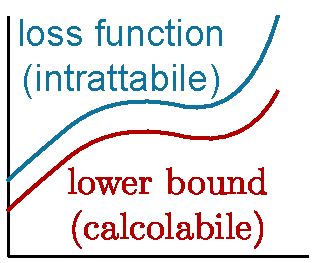
\includegraphics[keepaspectratio, scale=0.5]{lower_bound.pdf}
    \caption{\emph{Lower bound} di una funzione. Fonte~\cite{royBeginnerGuideDiffusion}.} 
    \label{fig:vlb}
\end{figure}
Invocando, ancora una volta, l'affinità intercorrente tra il processo di diffusione inversa e il decoder 
di un VAE, si può ricorrere al \emph{lower bound variazionale} (VLB) (o \emph{lower bound dell'evidenza} (ELBO)) che, 
declinato al contesto dei modelli di diffusione, è:
\begin{equation}
    \log \bigl(p_{\bm{\theta}}(\mathbf{x}_0)\bigr)\geq\underbrace{\mathbb{E}_q\biggl[\log\frac{p_{\bm{\theta}}(\mathbf{x}_{0:T})}{q(\mathbf{x}_{1:T}|\mathbf{x}_0)}\biggr]}_{VLB}
\end{equation}
(si veda Appendice~\ref{appendix:details_loss} per la derivazione dettagliata), e, come si vedrà nel prosieguo, risulterà essere trattabile. 
Pertanto, minimizzare la funzione di costo $L$ significa minimizzare il VLB cambiato di segno:
\begin{equation}
    L=-\log \bigl(p_{\bm{\theta}}(\mathbf{x}_0)\bigr)\leq L_{vlb}\triangleq\mathbb{E}_q\biggl[-\log\frac{p_{\bm{\theta}}(\mathbf{x}_{0:T})}{q(\mathbf{x}_{1:T}|\mathbf{x}_0)}\biggr]
\end{equation}
\begin{oss}
A rigore l'uso del pedice \emph{vlb} in $L_{vlb}$ è un abuso di notazione, dal momento che $L_{vlb}$ non è 
un lower bound ma è un \emph{upper bound} della funzione di costo $L$. Tuttavia, si predilige 
tale notazione $L_{vlb}$ per essere consistenti con la letteratura.
\end{oss}
\noindent A valle di una serie di calcoli che sono riportati in Appendice~\ref{appendix:details_loss} si perviene al seguente risultato:
\begin{equation}
    L_{vlb}=L_0+\sum_{t=2}^TL_{t-1}+L_T \label{eq:Lvlb}
\end{equation}
dove:
\begin{itemize}
    \item $L_0=-\log \bigl(p_{\bm{\theta}}(\mathbf{x}_0|\mathbf{x}_1)\bigr)$. Ho et al.~\cite{ho2020} hanno delegato ad un apposito decoder l'approssimazione di tale termine
    che, pertanto, può essere trascurato nella fase di addestramento della rete neurale.
    \item $L_{t-1}=D_{KL}\bigl(q(\mathbf{x}_{t-1}|\mathbf{x}_t,\mathbf{x}_0)\,\|\,p_{\bm{\theta}}(\mathbf{x}_{t-1}|\mathbf{x}_t)\bigr)$. L'obiettivo  
    è quello di addestrare la rete neurale, cosicché $p_{\bm{\theta}}(\mathbf{x}_{t-1}|\mathbf{x}_t)$ approssimi 
    quanto più fedelmente la distribuzione $q(\mathbf{x}_{t-1}|\mathbf{x}_t,\mathbf{x}_0)$ in 
    modo da minimizzare il termine $L_{t-1}$ (ricorrendo all'usuale interpretazione della \emph{divergenza di Kullback-Leibler} 
    (Appendice~\ref{appendix:details_loss},~\ref{eq:kullback-leibler})
    come una misura della distanza tra le distribuzioni).
    \item $L_T=D_{KL}\bigl(q(\mathbf{x}_T|\mathbf{x}_0)\,\|\,p(\mathbf{x}_T)\bigr)$ è un termine che può essere \emph{ignorato} durante 
    la fase di addestramento, dal momento che non annovera alcun parametro che possa essere appreso dalla rete neurale. 
    Infatti $p(\mathbf{x}_T)=q(\mathbf{x}_T)\sim\mathcal{N}(\bm{0},\bm{I})$ 
    e $q(\mathbf{x}_T|\mathbf{x}_0)$ è fissato una volta scelti gli iperparametri $\beta_t$~\eqref{eq:forward_diff_v2}.
\end{itemize}

\begin{oss}
    Definendo uno schema di diffusione opportuno (i.e.\ i valori dei $\beta_t$)
    e scegliendo l'iperparametro $T$ sufficientemente elevato, entrambe le distribuzioni 
    $q(\mathbf{x}_T|\mathbf{x}_0)$ e $p(\mathbf{x}_T)$ approssimano una gaussiana standard. 
    Quindi, stante l'interpretazione della divergenza di Kullback-Leibler come una misura della distanza tra tali distribuzioni,
    il termine $L_T=D_{KL}\bigl(q(\mathbf{x}_T|\mathbf{x}_0)\,\|\,p(\mathbf{x}_T)\bigr)$ tende a zero.
\end{oss}
\noindent Dunque, affinché $L_{vlb}$ risulti trattabile è sufficiente che $L_{t-1}$ ammetta un'espressione in forma chiusa.

\noindent Restringendo l'attenzione al termine $L_{t-1}$, 
in Appendice~\ref{sec:detailed_loss_term} si mostra che sussistono le seguenti considerazoni:
\begin{itemize}
\item poiché:
\begin{align}
    q(\mathbf{x}_{t-1}|\mathbf{x}_t,\mathbf{x}_0) &= \mathcal{N}(\mathbf{x}_{t-1}; \tilde{\bm{\mu}}_{t}(\mathbf{x}_t,\mathbf{x}_0),\tilde{\beta_t} \bm{I}) \label{eq:rif1}\\
    p_{\theta}(\mathbf{x}_{t-1}|\mathbf{x}_t)&=\mathcal{N}(\mathbf{x}_{t-1};\bm{\mu}_{\bm{\theta}}(\mathbf{x}_t,t),\bm{\Sigma}_{\bm{\theta}}(\mathbf{x}_t,t)) \label{eq:rif2}
\end{align}
segue che $L_{t-1}=D_{KL}\bigl(q(\mathbf{x}_{t-1}|\mathbf{x}_t,\mathbf{x}_0)\,\|\,p_{\theta}(\mathbf{x}_{t-1}|\mathbf{x}_t)\bigr)$ è 
la divergenza di Kullback-Leibler tra due gaussiane, e in quanto tale può essere espresso in forma chiusa. 
\item nella~\eqref{eq:rif2}, sebbene in linea di principio si possa addestrare 
la rete neurale ad apprendere sia $\bm{\mu}_{\bm{\theta}}(\mathbf{x}_t,t)$ che $\bm{\Sigma}_{\bm{\theta}}(\mathbf{x}_t,t)$, Ho et al.~\cite{ho2020} 
hanno \emph{fissato la varianza}  $\bm{\Sigma}_{\bm{\theta}}(\mathbf{x}_t,t)=\beta_t\bm{I}$. Quindi nella fase di addestramento 
la rete neurale deve apprendere la sola media $\bm{\mu}_{\bm{\theta}}(\mathbf{x}_t,t)$.
\item anziché addestrare la rete neurale ad apprendere, in ogni passo di diffusione inversa, la media $\bm{\mu}_{\bm{\theta}}(\mathbf{x}_t,t)$, 
si mostra che la rete può equivalentemente essere addestrata a predire il rumore $\bm{\epsilon}_{\bm{\theta}}(\mathbf{x}_t,t)$
che deve essere rimosso in ogni step della diffusione inversa per giungere all'immagine di partenza.
\end{itemize}

\noindent Stante i suddetti risultati, in Appendice~\ref{appendix:details_loss} si mostra che ognuno degli $L_{t-1}$ nella~\eqref{eq:Lvlb} 
assume la seguente forma semplificata:
\begin{equation}
    L_{t-1}^{\text{simple}}=\Vert \bm{\epsilon}-
    \bm{\epsilon}_{\bm{\theta}}(\underbrace{\sqrt{\overline{\alpha}_t}\mathbf{x}_0+\sqrt{1-\overline{\alpha}_t}\bm{\epsilon}}_{\mathbf{x}_t},t)\Vert^2 +C
    \label{eq:simple_loss}
\end{equation}
dove $C$ è una costante che non dipende da $\bm{\theta}$ e, quindi, può essere ignorata durante l'addestramento.

In definitiva, partendo da una funzione di costo $L=-\log\bigl(p_{\bm{\theta}}(\mathbf{x}_0)\bigr)$ intrattabile 
si è giunti alla~\eqref{eq:simple_loss}, in cui ognungo degli $L_{t-1}$ è, banalmente, l'\emph{errore quadratico medio} tra il rumore $\bm{\epsilon}$, aggiunto nella diffusione in avanti, e 
il rumore \emph{stimato} della rete neurale $\bm{\epsilon}_{\bm{\theta}}(\mathbf{x}_t,t)$.


\subsubsection{Architettura della rete neurale e algoritmo di addestramento}
Dal momento che la rete neurale deve fornire in uscita un'immagine (i.e.\ la stima del rumore), 
che è un \emph{tensore} avente le stesse dimensioni dell'immagine rumorosa in ingresso alla rete, 
Ho et al.~\cite{ho2020} hanno implementato la suddetta rete neurale con una U-Net, in virtù della sua peculiarità di produrre un'immagine 
con le medesime dimensioni dell'immagine in ingresso.
In Appendice~\ref{appendix:unet} sono riportati ulteriori dettagli sulla U-Net utilizzata in un DDPM.
\begin{algorithm}[H]
    \caption{Addestramento. Fonte~\cite{ho2020}}\label{alg:training}
   \begin{algorithmic}[1]
    \Repeat    
   \State $\mathbf{x}_0 \sim q(\mathbf{x}_0)$\label{row:training1}
    \State $t \sim \text{Uniform$(\{2,...,T\})$}$\label{row:training2}
   \State $\boldsymbol{\epsilon}\sim \mathcal{N}(\bm{0},\bm{I})$\label{row:training3}
   \State $\mathbf{x}_t=\sqrt{\overline{\alpha}_t}\mathbf{x}_0+\sqrt{1-\overline{\alpha}_t}\bm{\epsilon}$\label{row:training4}
   \State Take gradient descent step on
    \State $\qquad \nabla_{\bm{\theta}} \Vert \bm{\epsilon}-\bm{\epsilon_{\theta}}(\mathbf{x}_t,t) \Vert^2$\label{row:training5}
    \Until converged
   \end{algorithmic}
\end{algorithm}
\noindent In Figura~\ref{fig:training} è illustrato il meccanismo sotteso ad un passo dell'algoritmo di addestramento (Algoritmo~\ref{alg:training}) 
della rete neurale. Nell'Algoritmo~\ref{alg:training}:
\begin{figure}
    \centering
    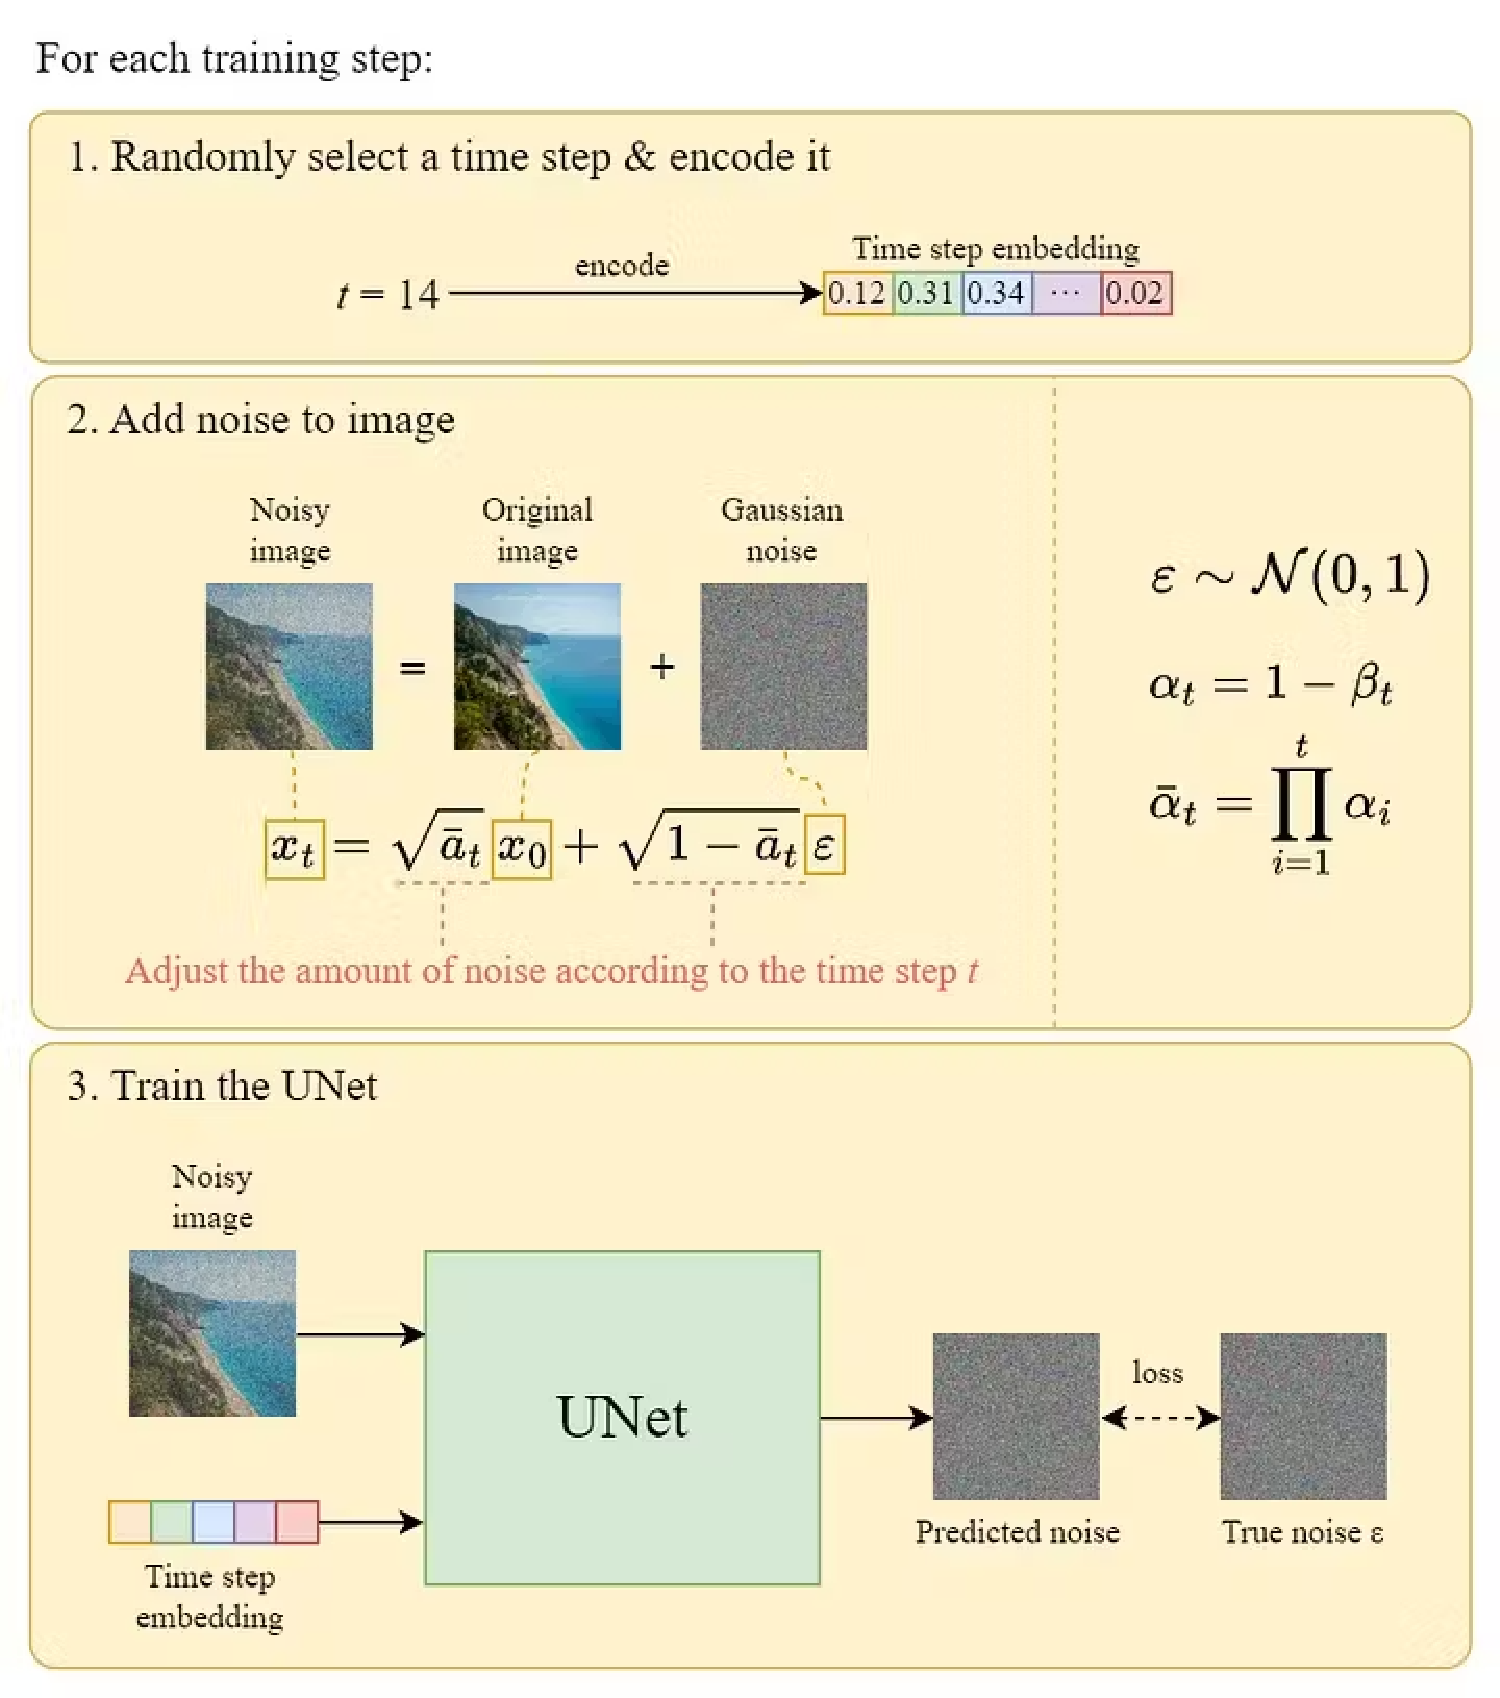
\includegraphics[keepaspectratio, scale=0.45]{training.pdf}
    \caption{Addestramento della rete neurale. Fonte~\cite{royBeginnerGuideDiffusion}.}
    \label{fig:training}
\end{figure}

\begin{itemize}
\item si considera un'immagine $\mathbf{x}_0$, nel dataset di addestramento, caratterizzata da una distribuzione incognita e arbitrariamente complessa $q(\mathbf{x}_0)$ (riga~\ref{row:training1}).
\item si seleziona \emph{a caso} (ciò giustifica il ricorso alla distribuzione uniforme) un passo temporale $t$ (riga~\ref{row:training2}).
\item si campiona del rumore $\bm{\epsilon}$ da una gaussiana standard (riga~\ref{row:training3}).
\item si applica il processo di diffusione in avanti nella sua versione ottimizzata~\eqref{eq:eff_forward}, per ottenere l'immagine rumorosa 
$\mathbf{x}_t$ a partire da $\mathbf{x}_0$ (riga~\ref{row:training4}).
\item si minimizzano i termini $L_{t-1}^{\text{simple}}=\Vert \bm{\epsilon}-\bm{\epsilon_{\theta}}(\mathbf{x}_t,t)\Vert^2$ 
con la tecnica del gradiente discendente stocastico (riga~\ref{row:training5}).
\end{itemize}

\begin{oss}
    Si noti come la riformulazione~\eqref{eq:eff_forward}  del processo di diffusione in avanti 
    permetta di scegliere \emph{a caso} il passo temporale $t$, e quindi il termine $L_{t-1}$ da ottimizzare, con il gradiente discendente, nella fase di 
    addestramento. 
\end{oss}











\subsection{Generazione di immagini}

Ultimato l'addestramento della U-Net, si possono sfruttare le transizioni~\eqref{eq:chain_transition132} della catena markoviana 
della diffusione inversa per rimuovere iterativamente il rumore.

In particolare, poiché la versione approssimata $\bm{\mu}_{\bm{\theta}}(\mathbf{x}_t,t)$, dalla rete neurale,
della media~\eqref{eq:true_mean} $\tilde{\bm{\mu}}_t(\mathbf{x}_t)$ è:
\begin{equation}
  \bm{\mu}_{\bm{\theta}}(\mathbf{x}_t,t)=\frac{1}{\sqrt{\alpha_t}}\biggl(\mathbf{x}_t-\frac{1-\alpha_t}{\sqrt{1-\overline{\alpha}_t}}\bm{\epsilon}_{\bm{\theta}}(\mathbf{x}_t,t)\biggr)\label{eq:learned_mean1}
\end{equation}
combinando la~\eqref{eq:learned_mean1} con la~\eqref{eq:chain_transition132}, e sfruttando l'artificio di riparametrizzazione~\eqref{eq:rep_trick}, risulta che 
\begin{equation}
  \mathbf{x}_{t-1}=\frac{1}{\sqrt{\alpha_t}}\biggl(\mathbf{x}_t-\frac{1-\alpha_t}{\sqrt{1-\overline{\alpha}_t}}\bm{\epsilon}_{\bm{\theta}}(\mathbf{x}_t,t)\biggr)+
  \sqrt{\beta_t}\bm{\epsilon} \label{eq:sampling}
\end{equation}
dove $\bm{\epsilon}$ è una gaussiana standard. 
Applicando ricorsivamente la formula~\eqref{eq:sampling} è possibile risalire, partendo da $\mathbf{x}_T$ 
(che è indistinguibile dal rumore puro), all'immagine di partenza $\mathbf{x}_0$ (Figura~\ref{fig:sampling}).

\medskip
\begin{oss}
A scopo puramente chiarificatore, si consideri, ad esempio, il passo $t=50$. 
Nella diffusione inversa il rumore $\bm{\epsilon}_{\bm{\theta}}(\mathbf{x}_{50},50)$, stimato dalla Unet, 
è il rumore che sottratto a $\mathbf{x}_{50}$ restituisce $\mathbf{x}_0$ non $\mathbf{x}_{49}$. 
Tuttavia, da un'attenta analisi della formula~\eqref{eq:sampling}, 
ciò che si sottrae a $\mathbf{x}_{50}$, per ottenere $\mathbf{x}_{49}$, è una versione scalata, 
del fattore $(1-\alpha_t)/\sqrt{1-\overline{\alpha}_t}$, di tale rumore.
\end{oss}

\smallskip
\begin{oss}
Avendo Ho et al.~\cite{ho2020} scelto uno schema di diffusione lineare, cosicché i $\beta_t$ si incrementano linearmente, 
e considerando le definizioni~\eqref{eq:alphas} di $\alpha_t$ e $\overline{\alpha}_t$, dalla formula~\eqref{eq:sampling} si evince che 
il primo passo della diffusione inversa sottrae da $\mathbf{x}_T$ soltanto una piccola parte del rumore $\bm{\epsilon}_{\bm{\theta}}(\mathbf{x}_t,t)$ stimato dalla U-Net.
Viceversa, i passi di diffusione inversa successivi sottraggono da $\mathbf{x}_t$ aliquote del rumore stimato dalla rete neurale via via sempre più grandi.
\end{oss}

\begin{figure}
\centering
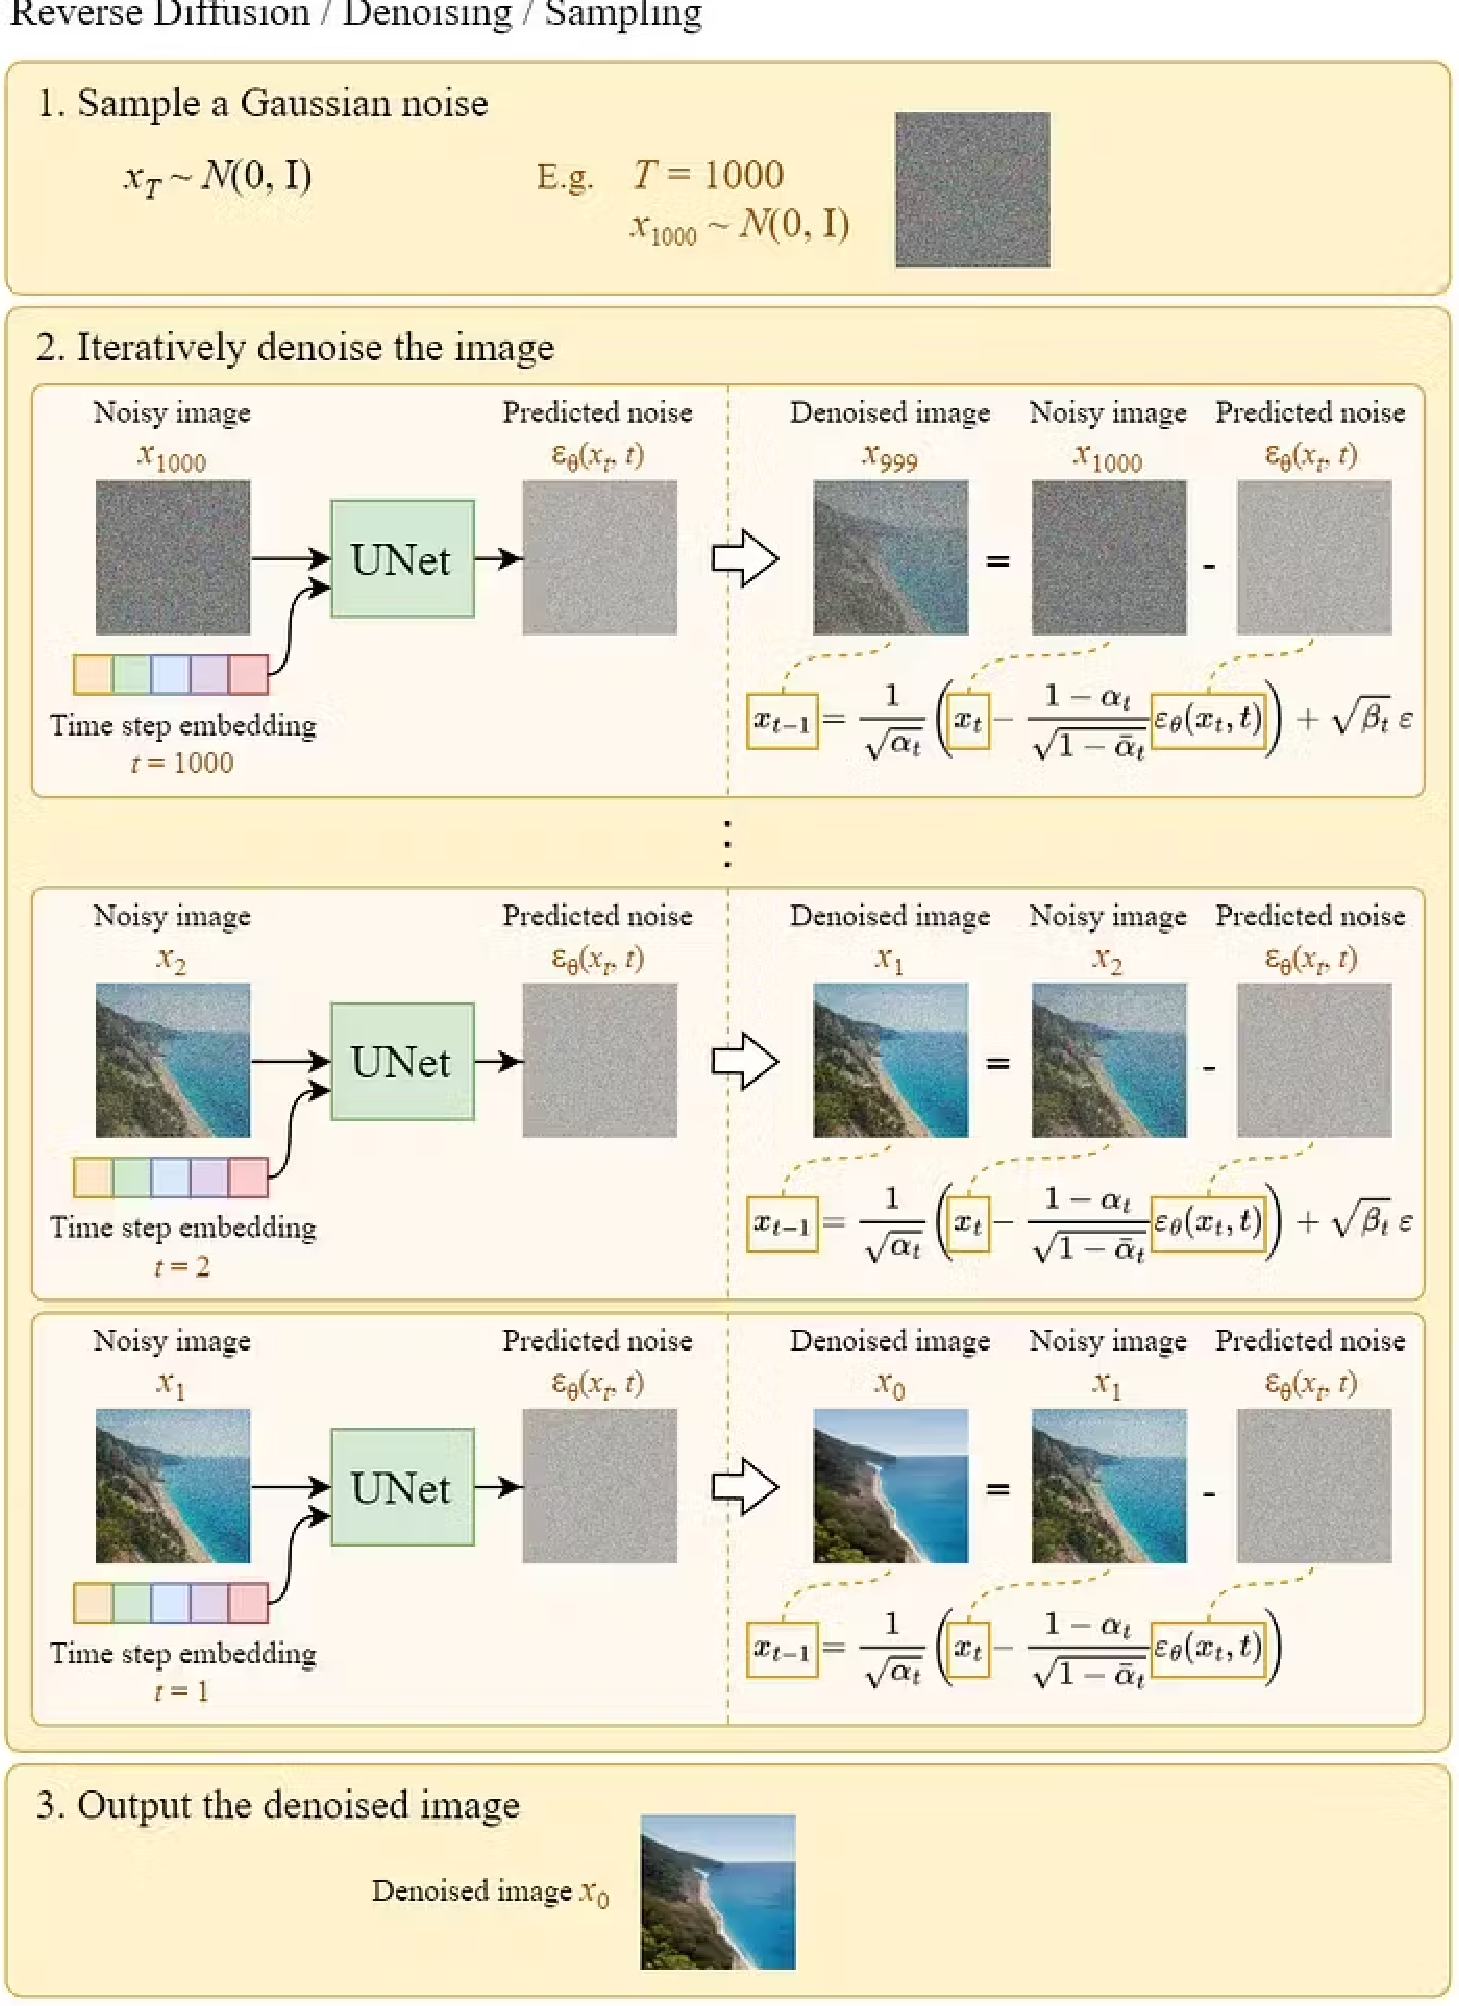
\includegraphics[keepaspectratio, scale=0.55]{sampling1.pdf}
\caption{Generazione di immagini con il processo di diffusione inversa. Fonte~\cite{royBeginnerGuideDiffusion}.}
\label{fig:sampling}
\end{figure}


\begin{algorithm}
    \caption{Generazione di immagini. Fonte~\cite{ho2020}}\label{alg:sampling}
   \begin{algorithmic}[1]
    \State $\mathbf{x}_T\sim\mathcal{N}(\bm{0},\bm{I})$
    \State \textbf{for} $t=T,\dots,1$ \textbf{do}
      \State \hspace{2em}$\mathbf{\bm{\epsilon}}\sim\mathcal{N}(\bm{0},\bm{I})$ if $t>1$, else $\mathbf{\bm{\epsilon}}=\bm{0}$
      \State \hspace{2em}$\mathbf{x}_{t-1}=\frac{1}{\sqrt{\alpha_t}}\biggl(\mathbf{x}_t-\frac{1-\alpha_t}{\sqrt{1-\overline{\alpha}_t}}\bm{\epsilon}_{\bm{\theta}}(\mathbf{x}_t,t)\biggr)+\sqrt{\beta_t}\mathbf{\bm{\epsilon}}$
    \State \textbf{end for}
    \State \textbf{return} $\mathbf{x}_0$
   \end{algorithmic}
\end{algorithm}

\subsection{Prestazioni}

A conclusione di tale capitolo vengono riportate le prestazioni del DDPM implementato da Ho et al.~\cite{ho2020},
misurate ricorrendo a due notorie metriche, ampiamente usate in letteratura, per valutare la qualità delle immagini prodotte da modelli generativi. 
Entrambe le due suddette metriche si avvalgono di una rete \emph{Inception-v3}~\cite{szegedyRethinkingInceptionArchitecture2015}, 
un classificatore di immagini pre-addestrato su ImageNet\footnote{\url{https://www.image-net.org/}}. In particolare:
\begin{itemize}
\item la metrica IS (\emph{Inception Score}) valuta la sola distribuzione delle immagini generate dal modello: 
ad un punteggio IS elevato corrisponde una migliore \emph{qualità} e \emph{varietà} delle immagini generate dal modello. 
\item la metrica FID (\emph{Fréchet Inception Distance}) confronta le distribuzioni delle immagini generate dal modello con quelle 
delle immagini del dataset di addestramento. Tale metrica, dal momento che “\emph{cattura la somiglianza delle immagini generate con quelle reali, 
meglio di quanto non faccia la metrica IS}”~\cite{heuselGANsTrainedTwo2017}, è lo standard \emph{de facto} per valutare la qualità delle immagini prodotte dai modelli generativi. 
Più basso è il il punteggio FID, più la distribuzione delle immagini generate si avvicina alla distribuzione delle immagini del dataset di addestramento.
\end{itemize}

\noindent Come già accennato in precedenza, Ho et al.~\cite{ho2020} hanno scelto $T=1000$ e hanno propeso, nel processo di diffusione in avanti, 
per uno schema di diffusione \emph{lineare}, con i $\beta_t$ che si incrementano linearmente da $\beta_1 = 10^{-4}$ a $\beta_T=0.02$. 
Gli iperparametri $\beta_t$, che implementano lo schema di diffusione, sono stati scelti molto più piccoli rispetto ai valori dei pixel delle immagini
di addestramento normalizzati tra $[-1, 1]$, cosicché le transizioni delle catene markoviane dei processi di diffusione diretta e inversa 
esibiscano approssimativamente la medesima forma funzionale (distribuzione gaussiana)
mantenendo, al contempo, il rapporto segnale rumore a valle della diffusione in avanti, il più contenuto possibile
($L_T=D_{KL}(q(\mathbf{x}_T|\mathbf{x}_0)\,\|\,\mathcal{N}(\bm{0},\bm{I})) \approx 10^{-5}$ bit per dimensione~\cite{ho2020}).

\noindent
Come si evince dalla Figura~\ref{fig:performance}, con un punteggio FID\footnote{i punteggi IS e FID riportati in Figura~\ref{fig:performance} sono stati calcolati su $50000$ campioni del dataset di addestramento CIFAR-10.} di $3.17$, 
il modello incondizionato addestrato da Ho et al.~\cite{ho2020} sul dataset CIFAR-10\footnote{Il dataset CIFAR-10 consiste di $60000$ immagini $32\times32$ a colori suddivise in 
$10$ classi, con $6000$ immagini per classe. Tale dataset annovera $50000$ immagini per l'addestramento e $10000$ per la fase di testing.} 
ottiene una migliore qualità dei campioni rispetto alla maggior parte dei modelli in letteratura, inclusa la classe dei modelli condizionali.



\begin{figure}[tp]
\centering
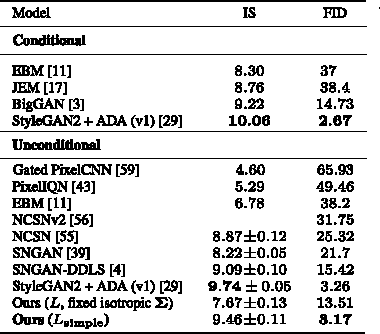
\includegraphics[keepaspectratio,scale=1.2]{performance.pdf}
\caption{Prestazioni DDPM. Fonte~\cite{ho2020}}\label{fig:performance}
\end{figure}
